\documentclass{article}
\usepackage[margin=2.9cm]{geometry} % Adjust the margin size here
\usepackage{graphicx}
% \usepackage{multirow}
\usepackage{tabularx}
\usepackage{hyperref}
\usepackage{csquotes}
\usepackage{enumerate}
\usepackage{parnotes}
\usepackage{natbib} % for bibliography
\usepackage{listings} % for code
\usepackage{tablefootnote}
\usepackage{xcolor}
\definecolor{codegreen}{rgb}{0,0.6,0}
\definecolor{codegray}{rgb}{0.5,0.5,0.5}
\definecolor{codepurple}{rgb}{0.58,0,0.82}
\definecolor{backcolour}{rgb}{0.95,0.95,0.92}
% \usepackage{footnote}
\lstdefinestyle{PythonStyle}{
    language=Python,
    basicstyle=\small\ttfamily,
    keywordstyle=\color{magenta},
    commentstyle=\color{codegreen},
    stringstyle=\color{blue},
    numbers=left,
    numberstyle=\tiny\color{purple},
    stepnumber=1,
    frame=single,
    breaklines=true,
    breakatwhitespace=false,
    tabsize=4,
    showspaces=false,
    showstringspaces=false
}
\newenvironment{itquote}
  {\begin{displayquote}\itshape}
  {\end{displayquote}\ignorespacesafterend}


\title{\vspace{-0.5cm}Project Plan }
\author{Joel Pointon\\Student ID: 10286413\\Course: MSc Data Science}
\date{\today}

\usepackage[acronym]{glossaries}
\makenoidxglossaries %\makenglossaries
\usepackage[acronym, toc]{glossaries}
\makenoidxglossaries %\makenglossaries
\newacronym{ai}{AI}{Artificial Intelligence}
\newacronym{faq}{FAQ}{Frequently Asked Question}
\newacronym{nlp}{NLP}{Natural Language Processing}
\newacronym{llm}{LLM}{Large Language Model}
\newacronym{cnn}{CNN}{Convolutional Neural Network}
\newacronym{rnn}{RNN}{Recurrent Neural Network}
\newacronym{ann}{ANN}{Artificial Neural Network}
\newacronym{lstm}{LSTM}{Long Short-Term Memory}
\newacronym{gru}{GRU}{Gated Recurrent Unit}
\newacronym{relu}{ReLu}{Rectified Linear Unit}
\newacronym{cbow}{CBOW}{Continuous Bag-of-Words}
\newacronym{elmo}{ELMo}{Embeddings from Language Model}
\newacronym{bert}{BERT}{Bidirectional Encoder Representations from Transformers}
\newacronym{bart}{BART}{Bidirectional and Auto-Regressive Transformer}
\newacronym{gpt}{GPT}{Generative Pre-trained Transformer}
\newacronym{sota}{SOTA}{state-of-the-art}
\newacronym{api}{API}{Application Programming Interface}
\newacronym{ram}{RAM}{Random-Access Memory}
\newacronym{glove}{GloVe}{Global Vectors for Word Representation}
\newacronym{squad}{SQuAD}{Stanford Question Answering Dataset}
\newacronym{mlm}{MLM}{Masked Language Modelling}
\newacronym{pdf}{PDF}{Portable Document Format}
\newacronym{cpu}{CPU}{central Processing Unit}
\newacronym{gpu}{GPU}{Graphics Processing Unit}
\newacronym{html}{HTML}{HyperText Markup Language}
\newacronym{rouge}{ROUGE}{Recall-Oriented Understudy for Gisting Evaluation}
\newacronym{bleu}{BLEU}{Bilingual Evaluation Understudy}
\newacronym{meteor}{METEOR}{Metric for Evaluation of Translation with Explicit ORdering}

\begin{document}

\maketitle
\section{Project Title}
An automated FAQ tool for Introduction to Image Processing module.
% Have You Tried Turning It Off and On Again? Pressing reset with a novel framework for the use of deep learning chatbots in education.

\section{Statement of the research problem} 
% Describe what the project is about and the particular the problem it seeks to address / solve. Outline why this is an interesting or important research problem that needs to be addressed / solved.
Inspired by ChatGPT \citep{ChatGPTrelease}, this project aims to create a ``framework/model'' that can automate the process of answering Frequently Asked Questions for the Introduction to Image Processing (COMP 2032) module. Generative chatbots such as ChatGPT can produce errors \citep{marcus2018, Bender21, Eva}, particularly when seeking to summarise documents \citep{Durmus_2020}. This means that students could be learning inaccurate or irrelevant information. Consequently, this paper aims to propose an efficient model for a domain-specific, knowledgeable Q\&A chatbot where tutors can have high confidence in the accuracy of any answers. This can free up academics so that they can spend their time more efficiently, to ``reinforce the learning of students'', improve their teaching methods \citep{Prez2020}, and ``focus on new experimental designs'' \citep{Eva}.

\section{Related work}
% Briefly discuss whether other people have done work on the same or similar problems in the past. Outline how your work builds on prior research and attempts to address / solve the problem. Describe how your approach is different and novel.
Transformers were introduced in \citeauthor{vaswani2017attention}'s `Attention Is All You Need' paper (\citeyear{vaswani2017attention}). The authors proposed a sequence-to-sequence model which uses 6 stacked encoders and decoders. The strength of Transformers lies in their ability to process all words in a sentence simultaneously, and their ability to retain context from much further back in the sequence \citep{vaswani2017attention}. There are multiple variations of the transformer architecture. The first is autoencoding (bidirectional) models which use stacked encoders (e.g. \acrshort{bert}: \citet{devlin2019bert}); the second is autoregressive (left-context) models which use stacked decoders (e.g. \acrshort{gpt}: \citet{radford2018improving}); the third is a combination of both, using both stacked encoders and decoders (e.g. \acrshort{bart}: \citet{lewis2019bart}), and these are known as sequence-to-sequence models.

There is little in the literature regarding attempting to produce (educational) chatbots by fine-tuning the above transformer models, however, Khan Academy is in the process of creating and trialling a knowledgeable tutor-bot using a fine-tuned version of \acrshort{gpt}-4 \citep{khanAcademy}. Unfortunately, \acrshort{gpt}-3.5-turbo and \acrshort{gpt}-4, which power ChatGPT \citep{ChatGPTrelease} are not publicly available for fine-tuning. Prior to the use of Transformer models, an alternative approach was used by \citet{Chen22} to create an extractive, domain-specific chatbot using a Deep \acrlong{cnn} (an \acrshort{lstm}-\acrshort{cnn} model), but this architecture cannot generate answers in natural language anywhere near as effectively. Therefore, this project seeks to provide a framework for a chatbot which can generate answers in natural language with a high degree of accuracy and reliability.

\section{Methodology}
% Outline how you are going to address / solve the research problem and evaluate your results. Describe the research techniques you will use (e.g., user studies, technology development, algorithm design, system implementation, lab experiments, etc.), and why these techniques are well suited to addressing / solving the problem.
This project will use several different AI models (both extractive and generative) in order to provide a holistic and comprehensive assessment of which model/framework is the most effective and appropriate. The four chosen models are \acrshort{bert}, \acrshort{bart}, and \acrshort{gpt}. Additionally, two \acrshort{gpt} models will be used - a pre-trained \acrshort{gpt}-2 model, and a fine-tuned \acrshort{gpt}-3.5-turbo model, so that different price \acrshort{gpt} models can be compared. This will also mean that any issues regarding insufficient model training data will be limited to only one or two of the above options.

To train the models, a knowledge base will need to be created from the module teaching resources, and cleaned into an appropriate format (e.g. Q\&A format) which can then be fed into the AI model. By using a pre-trained model (for \acrshort{bart} and \acrshort{gpt}), I can then fine-tune them to be knowledgeable about COMP 2032 using their neural network structure. This work will be resource-intensive, and issues could arise regarding sufficient computing power, so I will use a combination of the school's GPU cluster, Google Collab, and Kaggle to train the models. I will use Python to conduct this project, specifically using Google's HuggingFace library, along with PyTorch, TensorFlow, and OpenAI. 

Model evaluation will use a combination of developer testing, accuracy on Q\&A datasets such as \acrshort{squad} 1.0 and 2.0, cost-effectiveness, and ease of use. The model which has the best overall performance will be the basis for the chosen framework. 

\section{Programme of work}
% Divide your project up into a series of discrete but interrelated components or ‘work packages’. For each major component give it a name and number, describe the activity involved in accomplishing it, and end each activity description with a milestone or a goal to be achieved for that work package so that you will know how to measure when you have successfully completed that stage of the work programme. For example, 
The required work for the MSc Project has been split into eight Work Packages (WPs):
\begin{enumerate}[\textbf{WP-}1]
    \item \textit{Topic Selection}: Conduct preliminary research to identify gaps in existing knowledge, to refine the research question and find areas of research suggested in the literature. Milestone 1 (M1) - Research question selection completed.

     \item \textit{Literature Review}: Review the existing literature to connect different technologies and establish the current SOTA models in chatbot technology. Critically analyse key papers and identify gaps in the literature. Milestone 2 (M2) – Literature review draft completed.
    
     \item \textit{Research Design}: Determine the models to be compared and contrasted. Outline the methodology I will use to construct a chatbot. Also establish success criteria against which each model can be compared.  Milestone 3 (M3) - Methodology draft completed.
    
     \item \textit{Knowledge Framework}: Assemble a `knowledge' base for COMP 2032 and develop framework which can easily be applied and scaled up to other modules. This will be used to train the four models. Milestone 4 (M4) - Knowledge base created.
    
     \item \textit{Model Training}: The main aspect of the development project is to use the knowledge framework to train each of the four models. I will use the school's GPU cluster, Google Collab, and Kaggle to train each of the models. Milestone 5 (M5) - Model training completed.
    
     \item \textit{Model Comparison}: Determine the best model by comparing and contrasting the four models. A combination of performance metrics and developer testing will be employed to establish the most effective model. Milestone 6 (M6) - Model comparison completed.
    
     \item \textit{Writing and Drafting}: Begin writing the main body of the dissertation. This includes the implementation and evaluation of the models, along with revising and editing previous sections (literature review/methodology). Milestone 7 (M7) - First dissertation draft completed.
    
     \item \textit{Finalise Writeup and Presentation}: Use the dissertation first draft to create a presentation to demonstrate the chosen model and training process. Use the presentation creation process to refine the dissertation. Milestone 8 (M8) - Final dissertation and presentation completed.

\end{enumerate}

\section{Time plan}
% Map your milestones to a time plan that covers the PGT project period (see the PGT projects pages on Moodle); don’t forget to allocate time for writing up your dissertation in the plan. The plan may be in the form of a Gantt chart or any other suitable representation that clearly maps milestones to specific deadlines. Insert the time plan as image (no word count).
\begin{figure}[h!]
    \centering
    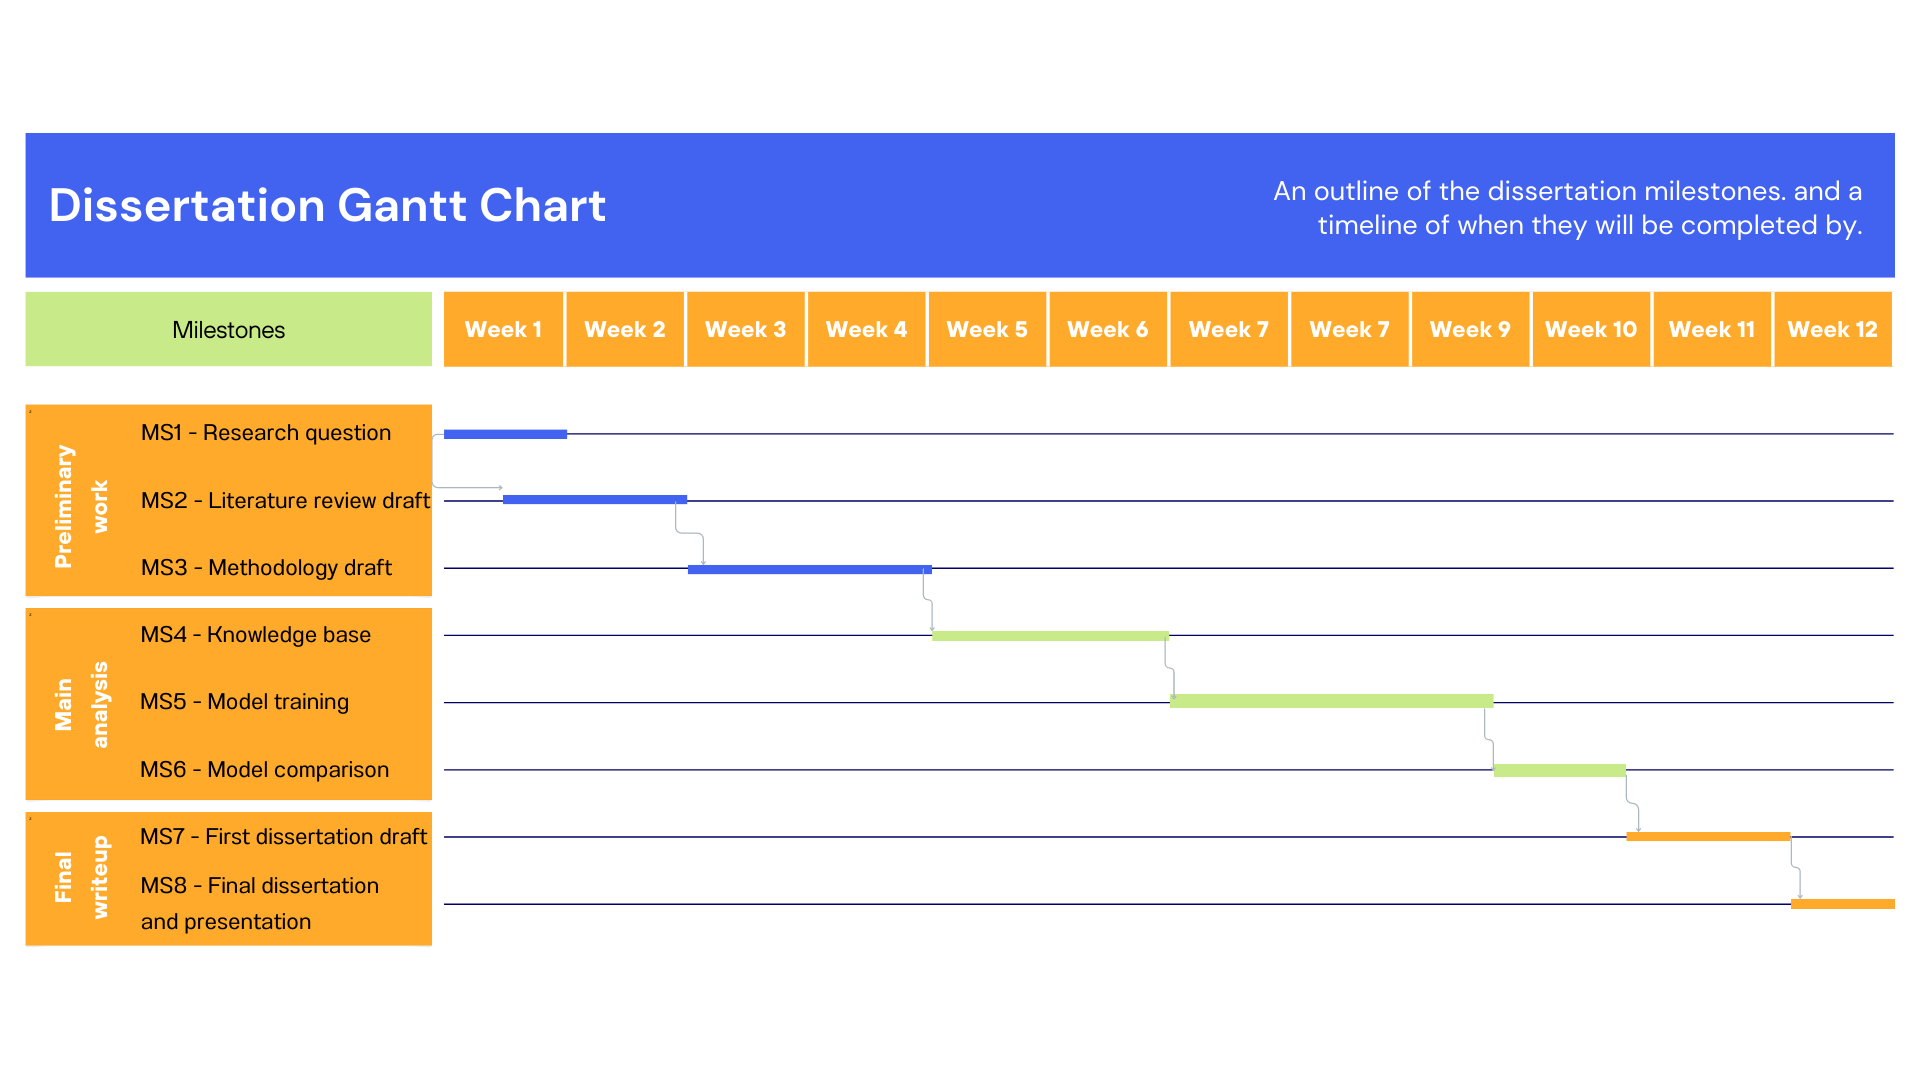
\includegraphics[width=0.95\textwidth,trim={0 3cm 0cm 0cm},clip]{paper/images/Diss Timeline.png}
    \caption{Completion Deadlines for Milestones}
    \label{fig:initial_framework}
\end{figure}

Word count out of 994/1000 words

% \pagebreak

\bibliographystyle{ecta} %for harvard
\bibliography{paper/bibliography/bibliography}

\noindent\makebox[\textwidth]{\rule{\textwidth}{0.4pt}}


\section{Assessment criteria}
Is there a clear statement of what the project is about?
\\*Is there an explanation of why this problem needs to be addressed / solved?
\\*Is the novelty of the proposed research substantiated with reference to related work?
\\*Is there a clear statement of how the problem is going to be addressed / solved?
\\*Are the proposed methods for addressing / solving the problem appropriate?
\\*Is there a clear statement of how the results are going to be evaluated?
\\*Is the proposed evaluation appropriate?
\\*Is there a breakdown of the research into work packages?
\\*Is this breakdown appropriate?
\\*Is there a time plan?
\\*Is the time plan realistic?
\newline
\\*Affirmative answers to each of these questions will result in a first class mark.  Markers should briefly describe how the project plan diverges from these desired outcomes to justify their mark.

\end{document}
